\documentclass{standalone}
\usepackage{tikz}
\usetikzlibrary{arrows,calc}

\begin{document}

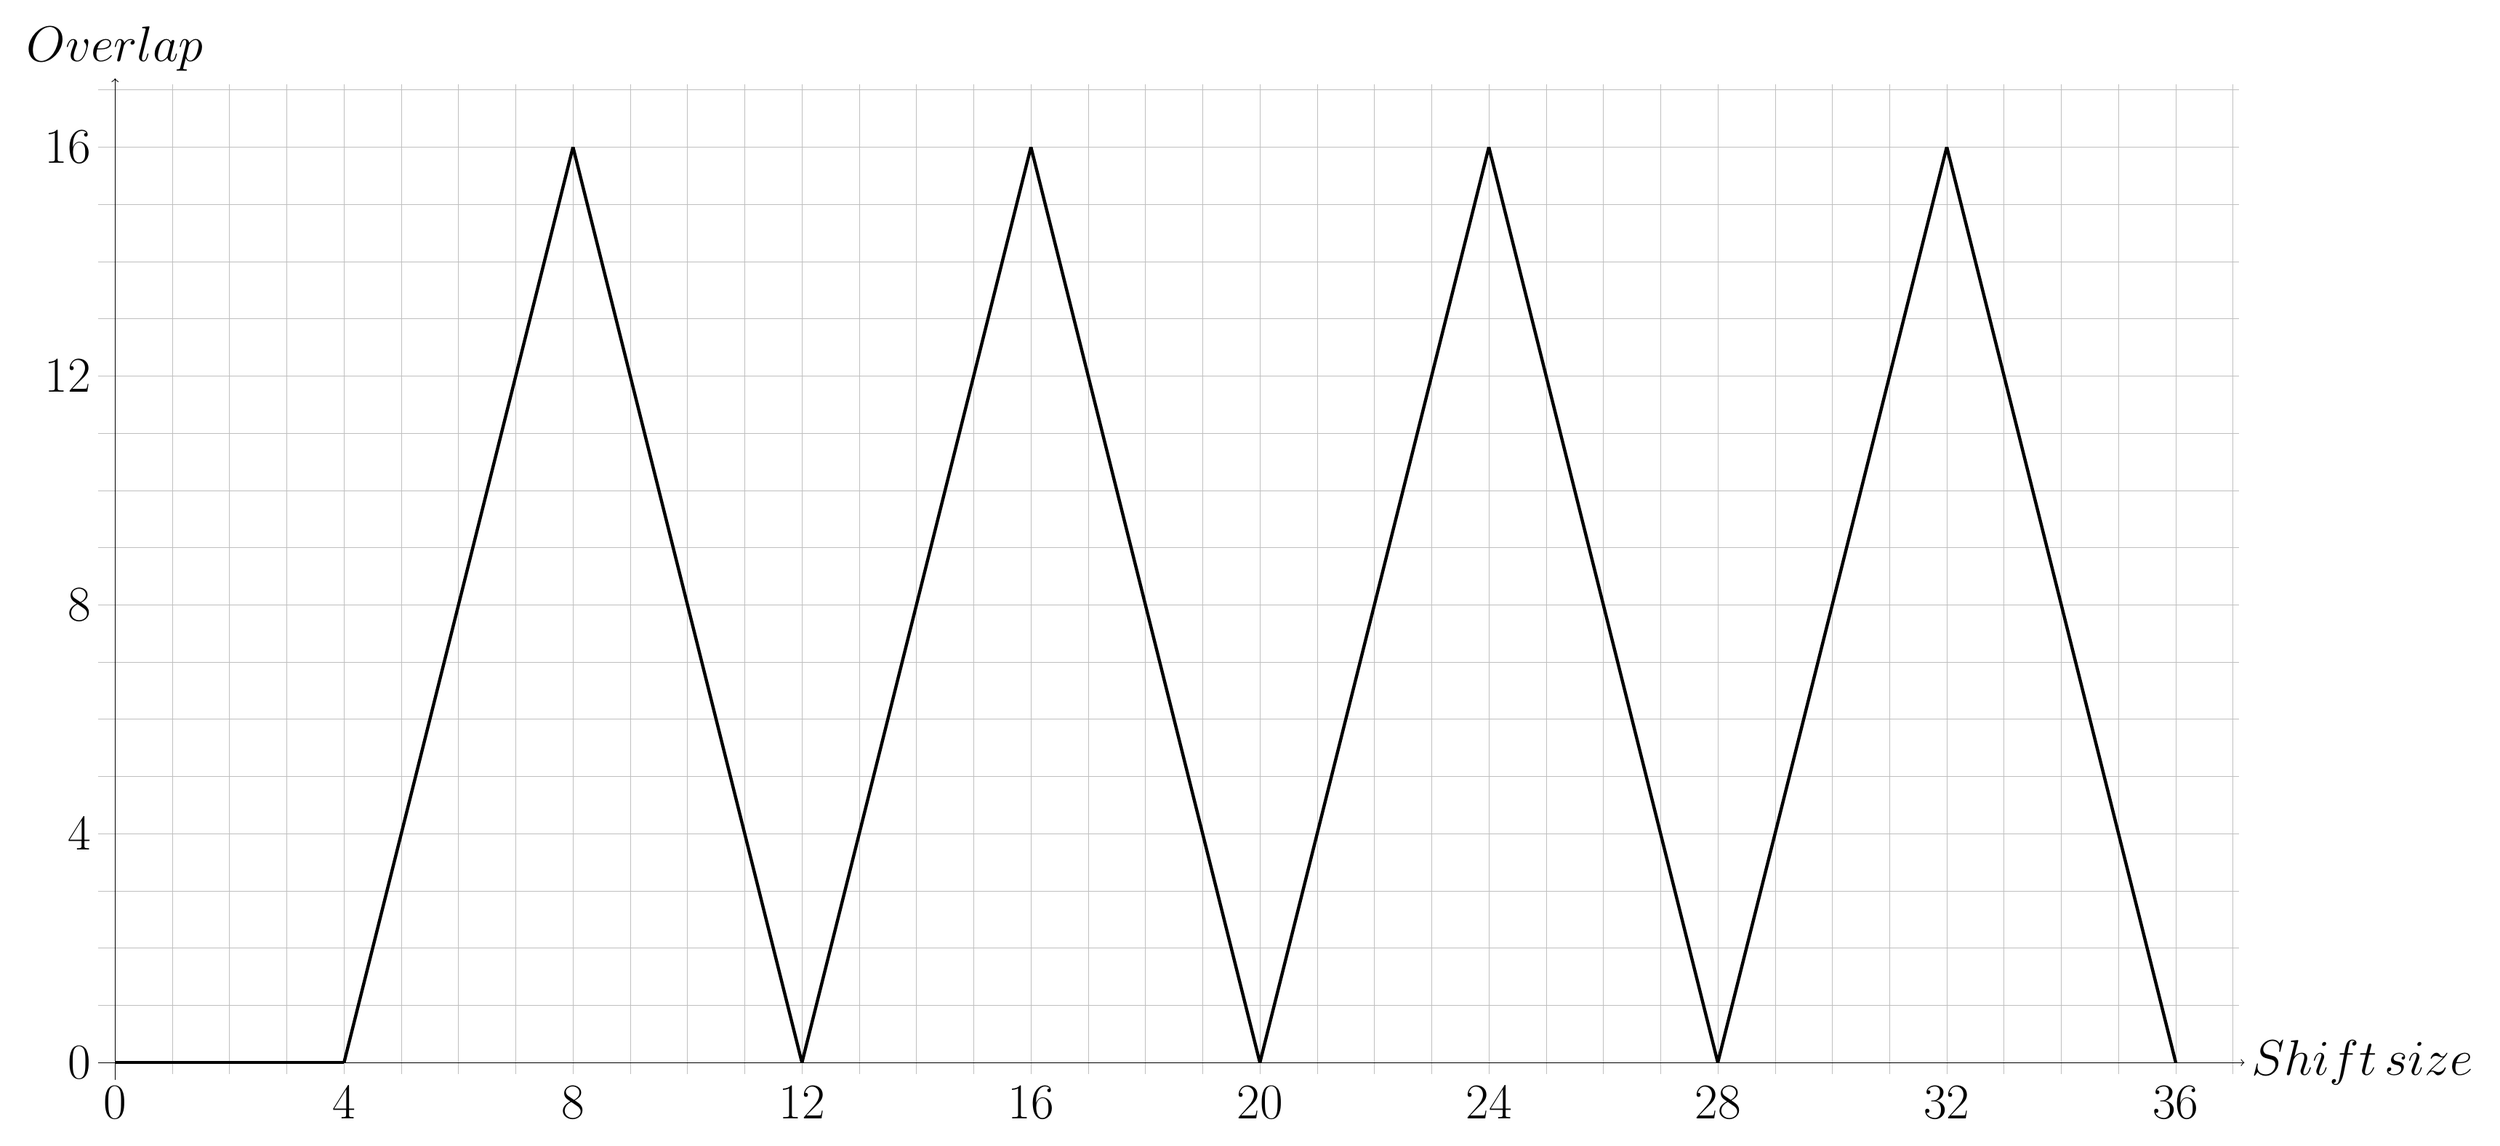
\begin{tikzpicture}
    \tikzstyle{every node}=[font=\Huge]

    \draw[very thin,color=gray!50] (-0.3,-0.2) grid (37.1,17.1);
    \draw[->] (-0.3,0) -- (37.2,0) node[right] {$Shift\thinspace size$};
    \draw[->] (0,-0.3) -- (0,17.2) node[above] {$Overlap$};
    \draw[-,ultra thick] (0,0) -- (4,0);
    \draw[-,ultra thick] (4,0) -- (8,16);
    \draw[-,ultra thick] (8,16) -- (12,0);
    \draw[-,ultra thick] (12,0) -- (16,16);
    \draw[-,ultra thick] (16,16) -- (20,0);
    \draw[-,ultra thick] (20,0) -- (24,16);
    \draw[-,ultra thick] (24,16) -- (28,0);
    \draw[-,ultra thick] (28,0) -- (32,16);
    \draw[-,ultra thick] (32,16) -- (36,0);

\foreach \x in {0,4,8,12,16,20,24,28,32,36}
 \node[anchor=north] at (\x,-0.3) {\x};
\foreach \y in {0,4,8,12,16}
 \node[anchor=east] at (-0.3,\y) {\y};

% \fill [radius=5pt] (4,0) circle [] (5,4) circle [] (6,8) circle []
% (7,12) circle [] (8,16) circle [] (9,12) circle [] (10,8) circle []
% (11,4) circle [] (12,0) circle;% \foreach \Point in {(-4,0), (-3,4), (-2,8), (-1
%,12), (0,16), (1,12),
%   (2,8), (3,4), (4,0)}{
%     \node at \Point {\textbullet};
% }


\end{tikzpicture}
\end{document} 
